% !TeX spellcheck = en_US
\chapter{Data Compression}

\section{Data Compression and Coding Fundamentals}
\subsection{Data Compression}
Uncompressed graphics, audio, and video data require substantial storage capacity, which is not possible in the case of uncompressed video data. The same is true for multimedia communications. Data transfer of uncompressed video data over digital networks requires that very high bandwidth be provided for a single point-to-point communication. To be cost-effective and feasible, multimedia systems must use compressed video and audio streams.

The most important compression techniques in use today are JPEG for single pictures, H.264 for video, MPEG for video and audio.


\subsection{Coding/Compression Fundamentals}
Images have considerably higher storage requirements than text, and audio and video have still more demanding properties for data storage. Moreover, transmitting continuous media also requires substantial communication data rates. The figures cited below clarify the qualitative transition from simple text to full-motion video data and demonstrate the need for compression. In order to be able to compare the different data⎄storage and bandwidth requirements of various visual media (text, graphics, images, and video), the following specifications are based on a small window of $ 640 \times 480 $ pixels on a display. The following holds always:
\begin{align*}
	& 1 \:kbit = 1000 \:bit  \\
	& 1 \:Kbit = 1024 \:bit  \\ 
	& 1 \:Mbit = 1024 \times 1024 \:bit &&
\end{align*}

\begin{enumerate}
	\item For the representation of the text medium, two bytes are used for every $ 8 \times 8 $ pixel character.
	% && is used to align equation to the left
\begin{flalign*}
	\textrm{Character per screen page} 
		& = {\frac{640 \times 480}{8 \times 8}} \\ 
		& = 4,800 &&
\end{flalign*}
\begin{flalign*}
	 	 \textrm{Storage required per screen page}  
		 	 	& = 4,800 \times 2 \: \textrm{byte} \\
				& = 9,600 \: \textrm{byte} \\
		 		& = 9.4 \: \textrm{Kbyte} &&
\end{flalign*}


\item For the representation of vector images, we assume that a typical image consists of $ 500 $ lines. Each line is defined by its coordinates in the $ x $ direction and
the $ y $ direction, and by an $ 8bit $ attribute field. Coordinates in the $ x $ direction require 10 bits$  (\log_2 (640) $), while coordinates in the $ y $ direction require $ 9 bits $
$ (log_2 (480) $).

\begin{flalign*}
\textrm{Bits per line} 
		&= 9\textrm{bits} + 10\textrm{bits} + 9\textrm{bits} + 10\textrm{bits} + 8\textrm{bits}\\
		& = 46 \textrm{bits} &&
\end{flalign*}
\begin{flalign*}
\textrm{Storage required per screen page} 
								& = 500 \times \frac{46}{8} \\
								& = 2,875 \: \textrm{byte} \\
								& = 2.8 \: \textrm{Kbyte} &&
\end{flalign*}	

\item Individual pixels of a bitmap can be coded using $ 256 $ different colors, requiring a single byte per pixel.
\begin{flalign*}
	\textrm{Storage required per screen page} 
	& = 640 \times 480 \times 1 \: \textrm{byte }\\
	& = 307,200 \: \textrm{byte} \\
	& = 300 \: \textrm{Kbyte} &&
\end{flalign*}

\end{enumerate}

The next examples specify continuous media and derive the storage required for one second of playback.

\begin{enumerate}
	\item Uncompressed speech of telephone quality is sampled at $ 8kHz $ and quantized using $ 8bit $ per sample, yielding a data stream of $ 64Kbit/s $.
	
	\begin{flalign*}
		\textrm{Required storage space/s}  
		& = \frac{64 \textrm{Kbit/s}}{8 \textrm{bit/byte}} \times \frac{1 \: \textrm{s}}{1,024 \: \textrm{byte/Kbyte}}\\
		& = 8 \: \textrm{Kbyte} &&
	\end{flalign*}

\item An uncompressed stereo audio signal of CD quality is sampled at $ 44.1kHZ $ and quantized using $ 16 bits $.

	\begin{flalign*}
	\textrm{Data rate}  
	& = 2 \times \frac{44,100}{s} \times \frac{16 \: \textrm{bit}}{8 \: \textrm{bit/byte}}\\
	& =  1, 76, 400 \: \textrm{byte/s} &&
\end{flalign*}

\item A video sequence consists of $ 25 $ full frames per second. The luminance and chrominance of each pixel are coded using a total of $ 3 bytes $.

According to the European PAL standard, each frame consists of $ 625 $ lines and has a horizontal resolution of more than $ 833 $ pixels. The luminance and color difference signals are encoded separately and transmitted together using a multiplexing technique $ (4:2:2) $.

According to CCIR 601 (studio standard for digital video), the luminance $ (Y) $ is sampled at $ 13.5MHz $, while chrominance ($ R - Y $ and $ B - Y $) is sampled using $ 6.75MHz $. Samples are coded uniformly using $ 8bits $.
\begin{flalign*}
	\textrm{Bandwidth}  
	& = (13.5 \textrm{MHz} + 6.75 \textrm{MHz}  + 6.75 \textrm{MHz})\times 8\textrm{bit}\\
	& = 216 \times 10^6 \:\textrm{bit/s} &&
\end{flalign*}
\begin{flalign*}
	\textrm{Data rate}  
	& = 640 \times 480 \times 25 \times 3 \: \textrm{bytes/s}\\
	& = 2,30,40,000 \:\textrm{byte/s} &&
\end{flalign*}
\begin{flalign*}
	\textrm{Required storage space/s}  
	& = 2,304 \times 10^4 \: \textrm{bytes} \times \frac{1 \: \textrm{s}}{1,024 \:\textrm{byte/Kbyte}}\\
	& = 22,500 \:\textrm{Kbyte} &&
\end{flalign*}
\end{enumerate}


\begin{landscape}
\subsubsection*{Classification of Coding/Compression Techniques}{\label{sec:compression-techniques}}
\begin{longtable}[c]{@{}p{5cm}p{8cm}p{5cm}@{}}
	\caption{Overview of some coding and compression techniques.}
	\label{tab:compression-techniques}\\
	\toprule
	\textbf{Coding Type}   & \textbf{Basis}  & \textbf{Technique} \\* \midrule
	\endfirsthead
	
	\multicolumn{3}{c}%
	{{\bfseries Table \thetable\ continued from previous page}} \\
	\toprule
	\textbf{Coding Type }   & \textbf{Basis}  & \textbf{Technique}  \\
	\endhead
	\endfoot
	
	\endlastfoot
	
	Entropy Coding & {Run-length Coding\par Huffman Coding\par  Arithmetic Coding\par}      \\
	\hline
	Source Coding  & {Prediction\par}   & {DPCM\par DM\par}           \\
	& Transformation\par  & FFT\par DCT\par \\
	
	& {Layered Coding (according to importance)\par}   & {Bit Position \par Subsampling\par Subband Coding\par }   \\
	& Vector Quantization\par & \\
	\hline

	Hybrid Coding  & {JPEG\par MPEG\par H.264\par}  &  \\
	 \bottomrule
\end{longtable}
\end{landscape}

%\begin{enumerate}
%	\item \textbf{Entropy Coding}
%		   \begin{itemize}
%		   	\item Run-length Coding
%		   	\item Huffman Coding
%		   	\item Arithmetic Coding
%		   \end{itemize}
%	   
%	\item \textbf{Source Coding}
%		 \begin{itemize}
%		 	\item Prediction
%		 	\item Transformation
%		 	\item Layered Coding
%		 	\item Vector Quantization
%		 \end{itemize}	
%	 
%	\item \textbf{Hybrid coding}
%		\begin{itemize}
%			\item JPEG
%			\item MPEG
%			\item H.264 (currently H.264)
%			\item Many proprietary systems
%		\end{itemize}
%\end{enumerate}



\section{Source, Entropy and Hybrid coding}
Compression techniques can be categorized as shown in Table \ref{tab:compression-techniques}. We distinguish among three types of coding: 
\begin{multicols}{3}
	\begin{enumerate}
		\item \textit{entropy},
		\item \textit{source}, and 
		\item \textit{hybrid} coding. 
	\end{enumerate}
\end{multicols}

Entropy coding is a lossless process, while source coding is often lossy. Most multimedia systems use hybrid techniques; most are only combinations of entropy and source coding, without any new processing algorithms.

\subsection{Entropy Coding}
\begin{itemize}
	\item Entropy coding is used regardless of the media's specific characteristics. 
	\item The data stream to be compressed is considered to be a simple digital sequence and the semantics of the data is ignored. 
	\item Entropy encoding is an example of \textit{lossless} encoding as the decompression process regenerates the data completely. 
	\item \textit{Run-length coding} is an example of entropy encoding that is used for data compression in file systems.
\end{itemize}


\subsection{Source Coding}

\begin{itemize}
	\item Source coding takes into account the semantics of the information to be encoded. 
	\item The degree of compression attainable with this often lossy technique depends on the medium. 
	\item In the case of lossy compression, a relation exists between the uncoded data and the decoded data; the data streams are similar but not identical. 
	\item In the case of speech, a considerable reduction of the amount of data can be achieved by transforming the time-dependent signal into the frequency domain, followed by an encoding of the formants\footnote{\textit{Formants} are defined as the maxima in the voice spectrum.}.
\end{itemize}





\subsection{Hybrid Coding}
To Understand the hybrid schemes, we consider a set of typical processing steps common to all techniques (entropy, source, and hybrid).

\subsubsection*{Major Steps of Data Compression}
Figure {\ref{fig:data-compression-steps}} shows the typical sequence of operations performed in the compression of still images and video and audio data streams. The following example describes the compression of one image:


\begin{enumerate}
	\item The \textit{preparation} step (here picture preparation) generates an appropriate digital	representation of the information in the medium being compressed. For example, a picture might be divided into blocks of $ 8 \times 8 \:pixels $ with a fixed number of bits per pixel.
	
	\item The \textit{processing} step (here picture processing) is the first step that makes use of the various compression algorithms. For example, a transformation from the time domain to the frequency domain can be performed using the Discrete Cosine Transform (DCT).
	
	\item \textit{Quantization} takes place after the mathematically exact picture processing step.
	
	\item \textit{Entropy coding} starts with a sequential data stream of individual bits and bytes.
\end{enumerate}


Figure {\ref{fig:data-compression-steps}} shows the compression process applied to a still image; the same principles can also be applied to video and audio data.

%%%%%%%%%%%%%%%%%%%%%%%%%%%%%%%%%%%%%%%%%
%										%
%				FIGURE				   	%
%										%
%%%%%%%%%%%%%%%%%%%%%%%%%%%%%%%%%%%%%%%%%
\begin{figure}[hb!]
	\centering
	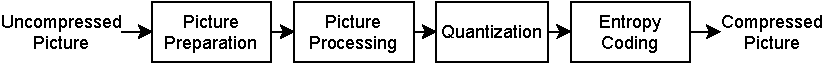
\includegraphics[width=0.9\textwidth]{data-compression-steps}
	\caption{Major steps of data compression.}{\label{fig:data-compression-steps}}
\end{figure}
%--------------------------Figure end -------------------

\textit{Decompression} is the inverse process of compression. Specific coders and decoders can be implemented very differently. Symmetric coding is characterized by comparable costs for encoding and decoding, which is especially desirable for dialogue applications. In an asymmetric technique, the decoding process is considerably less costly than the coding process. 

This is intended for applications where:
\begin{itemize}
	\item compression is performed once and 
	\item decompression takes place very frequently, or if the decompression must take place very quickly
\end{itemize}

For example, an audio-visual course module is produced once, but subsequently decoded by the many students who use it. The main requirement is real-time decompression. An asymmetric technique can be used to increase the quality of the compressed images.

\section{Basic Data Compression Techniques}
Compression basically employs redundancy in the data:
\begin{itemize}
	\item \textit{Temporal} in 1D data, 1D signals, audio, between video frames etc.
	\item \textit{Spatial} correlation between neighboring pixels or data items.
	\item \textit{Spectral} e.\ g.\ correlation between color or luminescence components. This uses the frequency domain to exploit relationships between frequency of change in data.
	\item \textit{Psycho-visual} exploit perceptual properties of the human visual system.
\end{itemize}

Compression methods can also be categorized in two broad ways:
\begin{enumerate}
	\item \textit{Lossless compression}:
	\begin{itemize}
		\item after decompression gives an exact copy of the original data.
		\item \textit{Example}: Entropy encoding schemes (Shannon-Fano, Huffman coding),	arithmetic coding, LZ/LZW algorithm (used in GIF image file format).
	\end{itemize}
	\item \textit{Lossy compression}:
		\begin{itemize}
		\item \textit{Example}: Transform coding — FFT/DCT based quantization used in	JPEG/MPEG differential encoding, vector quantization.
		\item Lossy methods are typically applied to high resolution audio, image compression.
		\item Have to be employed in video compression (apart from special cases).
	\end{itemize}
\end{enumerate}
 

%The hybrid compression techniques often used on audio and video data in multimedia systems are themselves composed of several techniques.
%
%The simplest techniques are based on \textit{interpolation} and \textit{subsampling}, whereby it is possible to make use of properties of the human eye or ear. For example, the eye is more sensitive to changes in brightness than to color changes. Therefore, instead of dividing an image into $ RGB $ (red, green, blue) components, a $ YUV $ representation can be used. The $ U $ and $ V $ components can then be sampled with lower horizontal and
%vertical resolution, a technique called \textit{subsampling}.

\subsection{Run-Length Coding}
\begin{itemize}
	\item Data often contains sequences of identical bytes. 
	\item By replacing these repeated byte sequences with the number of occurrences, a substantial reduction of data can be	achieved. 
	\item This is known as \textit{run-length coding}. 
\end{itemize}


A special marker $ M $ is needed in the data that does not occur as part of the data stream itself. 
To illustrate this, we define the exclamation mark `!' to be the `M-byte'. A single occurrence of an exclamation mark is interpreted as the `M-byte' during decompression. Two consecutive exclamation marks are interpreted as an exclamation mark occurring within the data.

The `M-byte' can thus be used to mark the beginning of a run-length coding. In the following example, the character \verb|C| occurs eight times in a row and is compressed to the three characters \verb|C!8| :

\[ \textrm{Uncompressed data:}\: \verb|ABCCCCCCCCDEFGGG|\]
\[ \textrm{Run-length coded:}\: \verb|ABC!8DEFGGG|\]


\subsection{Zero Suppression}
\begin{itemize}
	\item Run-length coding is a generalization of \textbf{zero suppression}, which assumes that just one symbol appears particularly often in sequences. 
	\item The blank (space) character in text is such a symbol; single blanks or pairs of blanks are ignored. 
\end{itemize}


\subsection{Pattern Substitution / Diatomic Encoding}
\begin{itemize}
	\item A technique that can be used for text compression substitutes single bytes for patterns that occur frequently. 
\end{itemize}


\subsection{Huffman Coding}
\begin{itemize}
	\item Huffman coding algorithm determines the optimal coding using the minimum number of bits. 
	\item Hence, the length (number of bits) of the coded characters will differ.
	\item The most frequently occurring characters are assigned to the shortest	code words. 
	\item A Huffman code can be determined by successively constructing a binary tree, whereby the leaves represent the characters that are to be encoded. 
	\item Every node contains the relative probability of occurrence of the characters belonging to the subtree beneath the node. 
	\item The edges are labeled with the bits $ 0 $ and $ 1 $.
\end{itemize}

\subsubsection*{Algorithm}
\begin{enumerate}
	\item Initialization: put all nodes in a list L, keep it sorted at all times (e.\ g.\ , ABCDE).
	\item Repeat until the list L has more than one node left.
	\begin{enumerate}[label=(\alph*)]
		\item From L pick two nodes having the lowest frequencies/probabilities, create a parent node of them.
		\item Assign the sum of the children’s frequencies/probabilities to the	parent node and insert it into L.
		\item Assign code 0/1 to the two branches of the tree, and delete the children from L
\end{enumerate}
\item Assign a codeword for each leaf based on the path from the root.
\end{enumerate}



%%%%%%%%%%%%%%%%%%%%%%%%%%%%%%%%%%%%%%%%%
%										%
%				FIGURE				   	%
%										%
%%%%%%%%%%%%%%%%%%%%%%%%%%%%%%%%%%%%%%%%%
\begin{figure}[ht!]
	\centering
	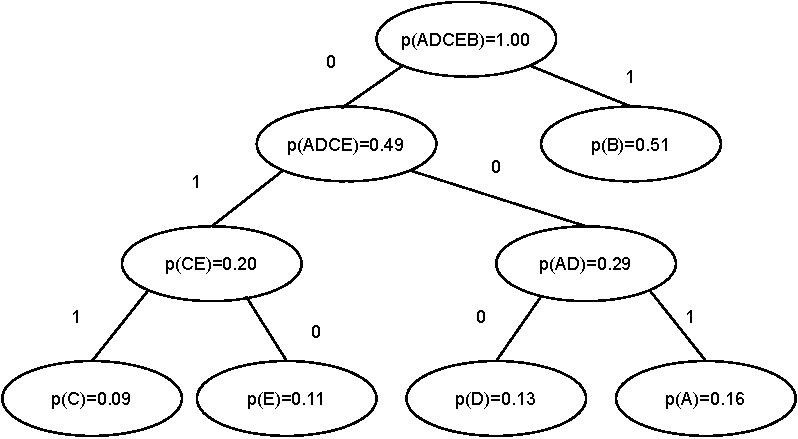
\includegraphics[width=0.8\textwidth]{huffman-coding}
	\caption{Example of a Huffman code represented as a binary tree}{\label{fig:huffman-coding}}
\end{figure}
%--------------------------Figure end -------------------

The following brief example illustrates this process:

\begin{enumerate}
	\item The letters $ A $, $ B $, $ C $, $ D $, and E are to be encoded and have relative probabilities of occurrence as follows:
	\[p(A)=0.16, p(B)=0.51, p(C)=0.09, p(D)=0.13, p(E)=0.11\]
	
	\item The two characters with the lowest probabilities, $ C $ and $ E $, are combined in the first binary tree, which gives the probability of $ 0.20 $ to their root node $ CE $. 
	
	\item Nodes with the following relative probabilities remain:
	\[p(A)=0.16, p(B)=0.51, p(CE)=0.20, p(D)=0.13\]
	
	The two nodes with the lowest probabilities are $ D $ and $ A $. These nodes are combined to form the leaves of a new binary tree. The combined probability of the
	root node $ AD $ is $ 0.29 $.
	
	
	\item Nodes with the following relative probabilities remain:
	\[p(AD)=0.29, p(B)=0.51, p(CE)=0.20\]
	
	The two nodes with the lowest probabilities are $ AD $ and $ CE $. These are combined into a binary tree. The combined probability of their root node $ ADCE $ is $ 0.49 $. 
	
	\item Two nodes remain with the following relative probabilities:
	\[p(ADCE)=0.49, p(B)=0.51\]
	
	These are combined to a final binary tree with the root node $ ADCEB $. 
	\item Figure {\ref{fig:huffman-coding}} shows the resulting Huffman code as a binary tree. The result is the following code words, which are stored in a table:
	\[w(A)=001, w(B)=1, w(C)=011, w(D)=000, w(E)=010\]
\end{enumerate}

Such a table could be generated for a single image or for multiple images together. The same table must be available for both encoding and decoding. 

\subsection{Arithmetic Coding}

\begin{itemize}
 \item Unlike Huffman coding, arithmetic coding does not code each symbol separately.
 \item Each symbol is instead coded by considering all prior data.
\end{itemize}

\subsection{Other Basic Techniques}
Apart from the compression techniques described earlier, some additional well
known techniques are used today:

\begin{itemize}
	\item Video compression techniques often use \textit{Color Look-Up Tables (CLUT)}.
	\item A simple technique for audio is silence suppression, whereby data is only encoded
	if the volume exceeds a certain threshold.
\end{itemize}

\section{Coding Standard JPEG, MPEG and DVI}

\subsection{JPEG}
\textit{Joint Photographic Experts Group (JPEG)} is an adaptive transformation coding techniques based on the Discrete Cosine Transform (DCT). In 1992, JPEG became an ISO International Standard. JPEG applies to color and gray-scaled still images.

Figure {\ref{fig:jpeg-compression-steps}} outlines the fundamental steps of JPEG compression in accordance with the general scheme illustrated in Figure {\ref{fig:data-compression-steps}}. JPEG defines several image compression modes by selecting different combinations of these steps.

\subsubsection*{JPEG Modes}
JPEG defines four modes, which themselves include additional variations:

\begin{itemize}
	\item The \textit{lossy}, sequential DCT-based mode (baseline process, base mode) must be
	supported by every JPEG decoder.
	\item The \textit{expanded lossy}, DCT-based mode provides a set of further enhancements to
	the base mode.
	\item The \textit{lossles}s mode has a low compression ratio and allows a perfect reconstruction
	of the original image.
	\item The \textit{hierarchical} mode accommodates images of different resolutions by using
	algorithms defined for the other three modes.
\end{itemize}

%%%%%%%%%%%%%%%%%%%%%%%%%%%%%%%%%%%%%%%%%
%										%
%				FIGURE				   	%
%										%
%%%%%%%%%%%%%%%%%%%%%%%%%%%%%%%%%%%%%%%%%
\begin{figure}[ht!]
	\centering
	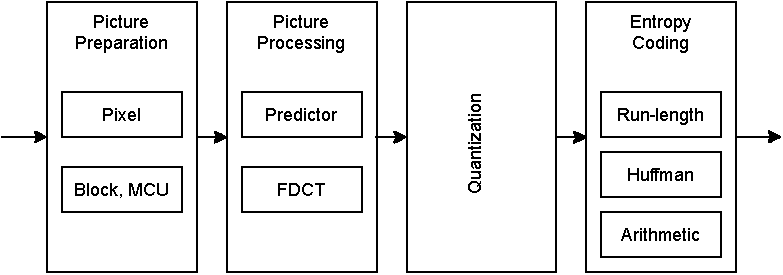
\includegraphics[width=0.8\textwidth]{jpeg-compression-steps}
	\caption[Steps of the JPEG compression technique]{Steps of the JPEG compression technique: summary of the different modes.}{\label{fig:jpeg-compression-steps}}
\end{figure}
%--------------------------Figure end -------------------



%\subsubsection{Image Preparation}
%For image preparation, JPEG specifies a very general image model that can
%describe most commonly used still image representations. For instance, the model is not
%based on three image components with $ 9-bit $ $ YUV $ coding and a fixed numbers of lines
%and columns. The mapping between coded color values and the colors they represent is
%also not coded. This fulfills the JPEG requirement of independence from image
%parameters such as image size or the image and pixel aspect ratios.
%
%An image consists of at least one and at most $ N=255 $ components or planes, as
%shown on the left side of Figure {\ref{fig:uncompressed-digital-image}}. These planes can be assigned to individual $ RGB $
%(red, green, blue) colors, or to the $ YIQ $ or $ YUV $ signals, for example.
%
%Each component is a rectangular array $ X_i \times Y_i $ of pixels (the samples). Figure {\ref{fig:jpeg-image-preparation}}
%shows an image with three planes, each with the same resolution.
%
%%%%%%%%%%%%%%%%%%%%%%%%%%%%%%%%%%%%%%%%%%
%%										%
%%				FIGURE				   	%
%%										%
%%%%%%%%%%%%%%%%%%%%%%%%%%%%%%%%%%%%%%%%%%
%\begin{figure}[H]
%	\centering
%	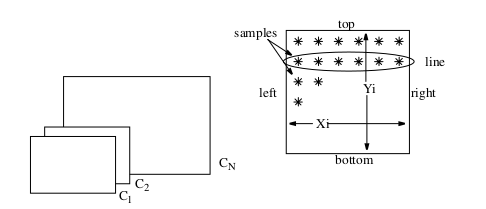
\includegraphics[width=0.8\textwidth]{uncompressed-digital-image}
%	\caption[Uncompressed digital image]{Digital uncompressed still image with the definition of the respective image components according to the JPEG standard}{\label{fig:uncompressed-digital-image}}
%\end{figure}
%%--------------------------Figure end -------------------
%
%The resolution of the individual components may be different. Figure {\ref{fig:jpeg-image-preparation-diff-res}} shows
%an image with three planes where the second and third planes have half as many columns as the first plane. A gray-scale image will, in most cases, consist of a single component, while an RGB color image will have three components with the same resolution (same number of lines $ Y_1 = Y_2 = Y_3  $and the same number of columns
%$ X_1 = X_2 = X_3 $ ). In JPEG image preparation, $ YUV $ color images with \textit{subsampling} of the
%chrominance components use three planes with $ Y_1 = 4Y_2 = 4Y_3 $ and $ X_1 = 4X_2 = 4X_3 $ .
%
%%%%%%%%%%%%%%%%%%%%%%%%%%%%%%%%%%%%%%%%%%
%%										%
%%				FIGURE				   	%
%%										%
%%%%%%%%%%%%%%%%%%%%%%%%%%%%%%%%%%%%%%%%%%
%\begin{figure}[H]
%	\centering
%	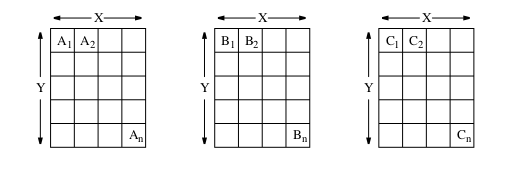
\includegraphics[width=0.8\textwidth]{jpeg-image-preparation}
%	\caption[Example of JPEG image preparation]{Example of JPEG image preparation with three components having the same resolution}{\label{fig:jpeg-image-preparation}}
%\end{figure}
%%--------------------------Figure end -------------------
%
%%%%%%%%%%%%%%%%%%%%%%%%%%%%%%%%%%%%%%%%%%
%%										%
%%				FIGURE				   	%
%%										%
%%%%%%%%%%%%%%%%%%%%%%%%%%%%%%%%%%%%%%%%%%
%\begin{figure}[H]
%	\centering
%	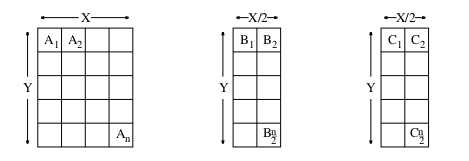
\includegraphics[width=0.8\textwidth]{jpeg-image-preparation-diff-res}
%	\caption[Example of JPEG image preparation having the different resolutions]{Example of JPEG image preparation with three components having the different resolutions}{\label{fig:jpeg-image-preparation-diff-res}}
%\end{figure}
%%--------------------------Figure end -------------------

\subsubsection*{Lossy Sequential DCT-Based Mode}
After image preparation, the uncompressed image samples are grouped into data units of $ 8 \times 8 $ pixels, as shown in Figure {\ref{fig:lossy-seq-dct}}; the order of these data units is defined by the MCUs. In this baseline mode, each sample is encoded using $ p=8bit $. Each pixel is an integer in the range $ 0 $ to $ 255 $.

%%%%%%%%%%%%%%%%%%%%%%%%%%%%%%%%%%%%%%%%%
%										%
%				FIGURE				   	%
%										%
%%%%%%%%%%%%%%%%%%%%%%%%%%%%%%%%%%%%%%%%%
\begin{figure}[h]
	\centering
	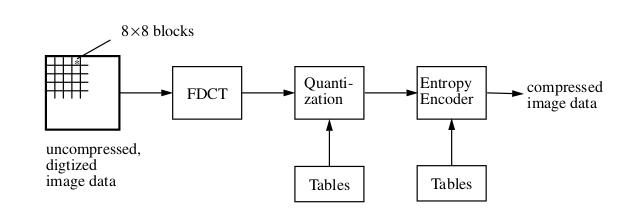
\includegraphics[width=\textwidth]{lossy-seq-dct}
	\caption[Steps of the lossy sequential DCT-based coding mode]{Steps of the lossy sequential DCT-based coding mode, starting with an
		uncompressed image after image preparation.}{\label{fig:lossy-seq-dct}}
\end{figure}
% --------------------------Figure end -------------------

%\paragraph*{Image Processing}
%The first step of image processing in the baseline mode, as shown in Figure {\ref{fig:lossy-seq-dct}}, is a transformation coding performed using the \textit{Discrete Cosine Transform (DCT)}. 

%The following \textit{FDCT (Forward DCT)} is then applied to each transformed pixel value:
%\[S_{vu}= \frac{1}{4}c_{u}c_{v}\sum_{x=0}^{7}\sum_{y=0}^{7}S_{yx}\cos \frac{(2x+1)u\pi}{16}\cos\frac{(2y+1)v\pi}{16}\]
%
%where, 
%\[c_{u}, c_{v}= \frac{1}{\sqrt{2}} \: \textrm{for} \: u, v=0; \: \textrm{otherwise}\: c_{u}, c_{v}=1\]
%
%Altogether, this transformation must be carried out 64 times per data unit. The result is $ 64 $ coefficients $ S_{vu} $.
%
%Due to the dependence of DCT on the Discrete Fourier
%Transform (DFT), which maps values from the time domain to the frequency domain,
%each coefficient can be regarded as a two-dimensional frequency.
%
%\subsubsection{Quantization}
%Image processing is followed by the quantization of all DCT coefficients; this is a
%lossy process. For this step, the JPEG application provides a table with 64 entries, one
%for each of the 64 DCT coefficients. This allows each of the 64 coefficients to be
%adjusted separately. The application can thus influence the relative significance of the
%different coefficients. Specific frequencies can be given more importance than others
%depending on the characteristics of the image material to be compressed. The possible
%compression is influenced at the expense of achievable image quality.
%
%The table entries $ Q_{vu} $ are integer values coded with $ 8 bits $. Quantization is
%performed according to the formula:
%\[sq_{vu}=round\frac{S_{vu}}{Q_{vu}}\]
%
%The greater the table entries, the coarser the quantization. Dequantization is per-
%formed prior to the IDCT according to the formula:
%\[R_{vu}=Sq_{vu} \times Q_{vu}\]
%Quantization and dequantization must use the same tables.
%
%\subsubsection{Entropy Encoding}
%During the next step, either the initial step of entropy encoding or preparation for
%the coding process, the quantized DC-coefficients are treated differently than the quan-
%tized AC-coefficients. The processing order of all coefficients is specified by the zig-zag
%sequence.
%
%JPEG uses Huffman coding and arithmetic coding as entropy encoding methods.
%For the lossy sequential DCT-based base mode, only Huffman
%encoding is allowed. In both methods, a run-length encoding of zero values is first
%applied to the quantized AC-coefficients. Additionally, non-zero AC-coefficients as
%well as the DC-coefficients are transformed into a spectral representation to further
%compress the data. The number of bits required depends on the value of each coefficient. Non-zero AC-coefficients are represented using between 1 and 10 bits. For the
%representation of DC-coefficients, a higher resolution of 1 bit to a maximum of 11 bits
%is used.

\paragraph*{Steps of JPEG Image Compression}
\begin{steps}
	\item \textit{Splitting}: The input image is divided into a small block which is having $ 8 \times 8 $ dimensions. This dimension is sum up to 64 units. Each unit of the image is called \textit{pixel}.
	\item \textit{Color Space Transform}: JPEG uses $ [Y,Cb,Cr] $ model instead of using the $ [R,G,B] $ model. $ RGB $ is converted into $ YCbCr $.
	\begin{itemize}
		\item Y is for brightness, 
		\item Cb is color blueness, and 
		\item Cr for color redness. 
	\end{itemize}
	\item \textit{Apply DCT}: After the conversion of colors, it is forwarded to DCT. DCT uses a cosine function and does not use complex numbers. It converts information which are in a block of pixels from the spatial domain to the frequency domain.
	\item \textit{Quantization}  is used to reduce the number of bits per sample.
	\item \textit{Serialization}: The zigzag scan is used to map the $ 8 \times8 $ matrix to a $ 1 \times 64 $ vector. Zigzag scanning is used to group low-frequency coefficients to the top level of the vector and the high coefficient to the bottom. 
	\item \textit{Vectoring}: The different pulse code modulation (DPCM) is applied to the DC component. DPCM encodes the difference between the current block and the previous block.
	\item \textit{Encoding}: Run Length Encoding (RLE) is applied to AC components. This is done because AC components have a lot of zeros in it. It encodes in a pair of \texttt{(skip, value)} in which \texttt{skip} is non-zero value and \texttt{value} is the actual coded value of the non-zero components.	
\end{steps}

\subsection{MPEG}
MPEG was developed and defined by ISO/IEC JTC1/SC 29/WG 11 to cover motion video as well as audio coding. 


\subsubsection{Video Encoding}
MPEG supports four types of image coding. In order to achieve a high compression ratio, temporal redundancies of successive images need to be exploited. Fast random access requires that images be coded individually. Hence the following image types are distinguished:

\paragraph{I-Frames (Intra-coded frames)}
%P-frames (predictive-coded frames)
	\begin{itemize}
	\item Are coded without using information about other frames.
	\item An $ I $-frame is treated as a still image. Here, MPEG	falls back on the results of JPEG.
	\item Unlike JPEG, real-time compression must be possible.
	\item The compression rate is thus the lowest within MPEG. 
	\item $ I $-frames form the anchors for random access.
	\item $ I $-frames are encoded by performing a DCT on the $ 8\times8 $ blocks defined within the macro blocks.
	\end{itemize}




\paragraph{P-Frames (Predictive-coded frames)}
\begin{itemize}
	\item Require information about previous I and/or $ P $	frames for encoding and decoding. 
	\item Decoding a $ P $-frame requires decompression of the last $ I $ frame and any intervening $ P $-frames. 
	\item In return, the compression ratio is considerably higher than for I frames. 
	\item A $ P $-frame allows the following $ P $-frame to	be accessed if there are no intervening $ I $ frames.
\end{itemize}


\paragraph{B-frames (Bidirectionally predictive-coded frames}
\begin{itemize}
	\item Require information from previous and following $ I $ and/or $ P $ frames. 
	\item $ B $-frames yield the highest compression ratio attainable in MPEG. 
	\item A $ B $-frame is defined as the difference from a prediction based on a previous and a following $ I $ or $ P $-frame. 
	\item It cannot serve as a reference for prediction coding of other frames.
\end{itemize}


\paragraph{D-frames (DC coded frames}
\begin{itemize}
	\item Are intraframe-coded and can be used for efficient fast forward. 
	\item During the DCT, only the DC-coefficients are coded; the AC coefficients are ignored.
\end{itemize}





\noindent Figure \ref{fig:mpeg-frames} shows a sequence of $ I $, $ P $, and $ B $-frames. This example illustrates the prediction for the first $ P $-frame and the bidirectional prediction for a $ B $-frame. The order in which the images are presented differs from the actual decoding order if $ B $-frames are present in an MPEG-coded video stream.


The pattern of $ I $, $ P $, and $ B $-frames in a sequence is determined by the MPEG application. For random access, the ultimate resolution would be attained by encoding the
entire stream using $ I $-frames. The highest compression rate can be achieved by using as many $ B $-frames as possible. For practical applications, the sequence \verb|IBBPBBPBBIBBPBBPBB...| has proven to be useful. This permits random access with a resolution of nine still images (i.\ e.\ , about $ 330ms $) and still provides a very good compression ratio. Every 15 images includes one $ I $-frame.

%%%%%%%%%%%%%%%%%%%%%%%%%%%%%%%%%%%%%%%%%
%										%
%				FIGURE				   	%
%										%
%%%%%%%%%%%%%%%%%%%%%%%%%%%%%%%%%%%%%%%%%
\begin{figure}[ht!]
	\centering
	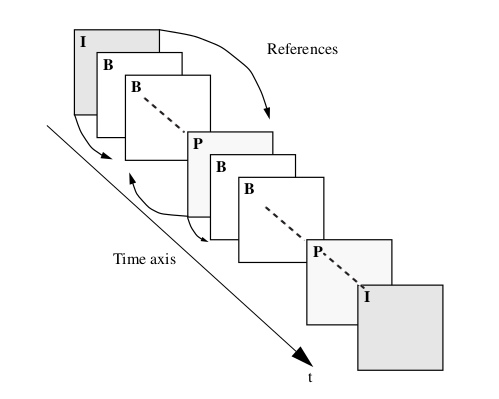
\includegraphics[width=0.7\textwidth]{mpeg-frames}
	\caption[Types of individual images in MPEG]{Types of individual images in MPEG: I, B, and P frames.}{\label{fig:mpeg-frames}}
\end{figure}
%--------------------------Figure end -------------------


%\subsubsection*{Quantization}
%Concerning quantization, it should be noted that AC-coefficients of $ B $ and $ P $-frames are usually very large values, whereas those of $ I $-frames are very small. Thus,
%MPEG quantization adjusts itself accordingly. If the data rate increases too
%much, quantization becomes more coarse. If the data rate falls, then quantization is
%performed with finer granularity.

\subsubsection{Audio Coding}
MPEG audio coding uses the same sampling frequencies as Compact Disc Digital Audio (CD-DA) and Digital Audio Tape (DAT), i.\ e.\ , $ 44.1 kHz $ and $ 48 kHz $, and additionally, $ 32kHz $ is available, all at $ 16 bits $.

Three quality levels (layers) are defined with different encoding and decoding complexity. An implementation of a higher layer must be able to decode the MPEG audio signals of lower layers.

%\paragraph*{Psychoacoustic Model}
%The noise level in each sub-band is determined using a psycho-acoustic model.

Similar to two-dimensional DCT for video, a transformation into the frequency domain is applied for audio. The Fast Fourier Transform (FFT) is a suitable technique.
As shown in Figure \ref{fig:mpeg-audio-encoding}:
\begin{itemize}
	\item The relevant portion of the spectrum is divided into 32 non-overlapping subbands. 
	\item The audio signal is thus split into 32 subbands. 
	\item Different components of the spectrum can then be quantized differently. 
	\item In parallel with the actual FFT,the noise level in each subband is determined using a psychoacoustic model. 
	\item At a higher noise level, a coarser quantization is performed. 
	\item A lower noise level results in finer quantization.
	\item In the first and second layers, the appropriately quantized spectral components are simply PCM-encoded. 
	\item The third layer additionally performs Huffman	coding.
\end{itemize}

\begin{figure}[ht!]
	\centering
	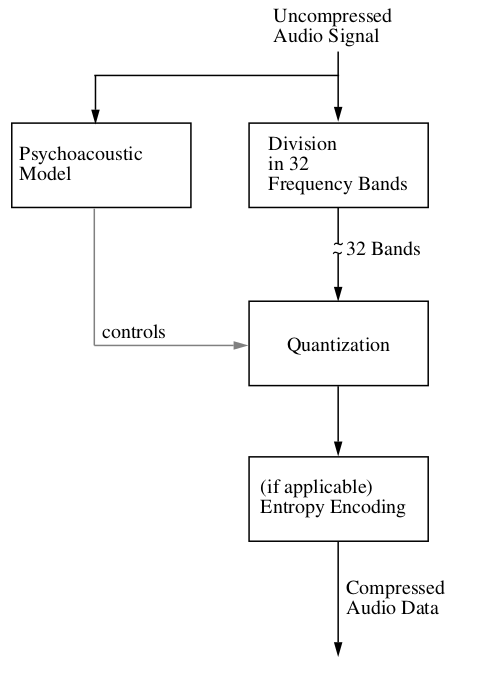
\includegraphics[width=0.6\textwidth]{mpeg-audio-encoding}
	\caption{MPEG audi encoding.}
	\label{fig:mpeg-audio-encoding}
\end{figure}

Audio coding can be performed on stereo sound, a single channel, or two independent channels. MPEG provides for two types of stereo sound. 
\begin{itemize}
	\item In the first case, two channels are processed completely independently. 
	\item In the joint stereo mode, MPEG achieves a higher compression ratio by exploiting redundancies between the two	channels.
\end{itemize}

\subsection{DVI}
\textit{Digital Video Interactive}(DVI) is a technology that includes coding algorithms. The fundamental components are a VLSI chip set for the video subsystem, a well-specified data format for audio and video files, an application user interface to the audio-visual kernel (AVK, the kernel software interface to the DVI hardware) and compression, as well as decompressing, algorithm. 

DVI can process\textit{ data, text, graphics, still images, video} and \textit{audio}. The original essential characteristic was the asymmetric technique of video compression and decompression known as Presentation-Level Video (PLV).

\subsubsection{Audio and Still Image Encoding}
Audio signals are digitized using $ 16 bits $ per sample and are either PCM-encoded or compressed using the Adaptive Differential Pulse Code Modulation (ADPCM) technique. Thereby, a reduction to about four bits per sample is achieved at a quality corresponding to stereo broadcasting.

When encoding still images, different video input formats can be used. These can be composite, as well as component video signals like, RGB. In the case of an RGB signal, the color of each pixel is split into portions of the three colors of the spectrum-red, green and blue - and each color is processed separately.

\subsubsection{Video Encoding}
For motion video encoding DVI distinguishes two techniques with different resolutions and dissimilar goals:

\begin{itemize}
	\item \textit{Presentation-Level Video (PLV)} is characterized by its better quality. This is achieved at the expense of a very time-consuming asymmetric compression
	performed by specialized compression facilities.
	
	\item \textit{Real-Time Video (RTV)} is a symmetric compression technique that works with hardware and software and can be performed in real-time.
\end{itemize}


Where,
\begin{enumerate}
	\item \textit{Asymmetric coding} requires considerably more effort for encoding than for decoding. Compression is carried out once, whereas decompression is performed many times. A typical application area is retrieval systems. 
	
	\item \textit{Symmetric compression} is characterized by a comparable effort for the compression and decompression processing.
\end{enumerate}
